Thinking...
The user asks: translate Japanese sentence to English, but keep TeX code as is. The Japanese text is:

"以下のの日本語文を英訳してください。ただしTeXのコードが挿入されているのでその部分はそのまま出力してください： \begin{figure}[h] \begin{center} 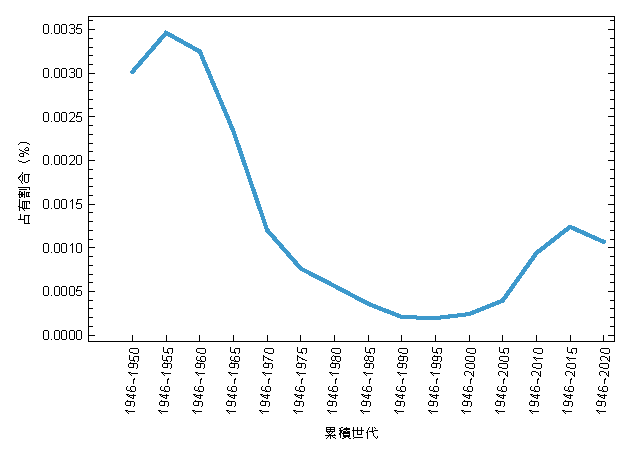
\includegraphics[width=76mm]{gr4.eps} \caption{高被引用論文の全論文に占める割合（\%）} \label{fig:gr4} \end{center} \end{figure}"

We need to translate the Japanese sentence (the instruction) into English? Actually the user says: "以下のの日本語文を英訳してください。" They want to translate the Japanese text that follows (the TeX code). So the Japanese text is likely the caption "高被引用論文の全論文に占める割合（\%）". The rest is LaTeX commands.

Thus output should be the same LaTeX code, but with the caption translated: "Proportion of highly cited papers among all papers (%)". Or something like that. Let's translate: "高被引用論文の全論文に占める割合（\%）" => "Percentage of highly cited papers among all papers (%)". Or "Proportion of highly cited papers in all papers (%)". Better: "Proportion of highly cited papers among all papers (%)". Keep \% as is.

Thus final output: same code but caption replaced.

We need to output only the code? The instruction says "その部分はそのまま出力してください" meaning keep TeX code unchanged, but we need to translate the Japanese part. The Japanese part inside caption is the only Japanese text. So we replace caption text with English translation.

Thus answer:

\begin{figure}[h]
\begin{center}
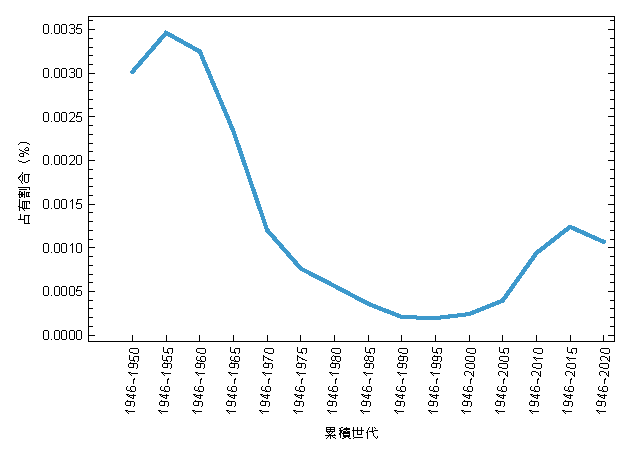
\includegraphics[width=76mm]{gr4.eps}
\caption{Proportion of highly cited papers among all papers (\%)}
\label{fig:gr4}
\end{center}
\end{figure}

We should not add any extra commentary.
...done thinking.

\begin{figure}[h]
\begin{center}
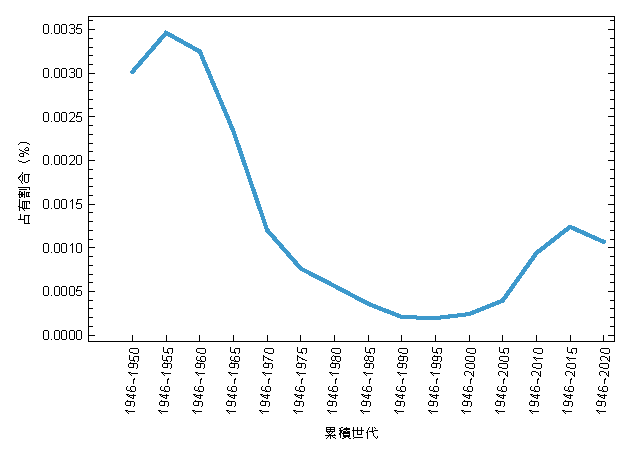
\includegraphics[width=76mm]{gr4.eps}
\caption{Proportion of highly cited papers among all papers (\%)}
\label{fig:gr4}
\end{center}
\end{figure}

